%!TEX root = Slic3r-Manual.tex

If the 3D mesh described in the model contains holes, or edges are misaligned (known as being non-manifold), then Slic3r may have problems working on it.  Slic3r will attempt to fix any problems it can, but some problems are out of its reach.  If the application complains that a model cannot be sliced correctly then there are several options available, and the ones described here are all free at the time of writing.

\paragraph{\texttt{FreeCAD}} % (fold)
\label{par:freecad}
\index{FreeCAD}

Freecad\footnote{http://sourceforge.net/projects/free-cad} is a comprehensive, and free, CAD program which comes with a mesh module, in which repairs to degenerate models can be made.  The following steps outline how a problem model file can be analysed and repaired.

\begin{figure}[H]
\centering
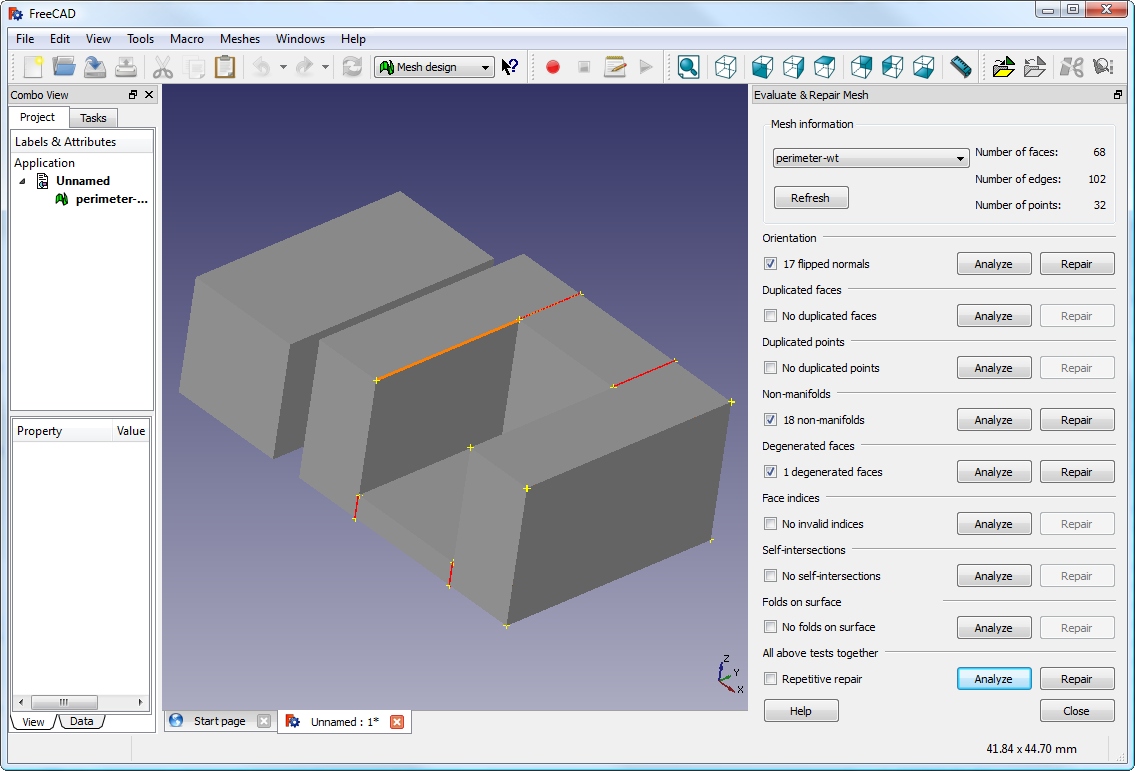
\includegraphics[keepaspectratio=true,width=0.75\textwidth]{working_with_models/freecad_part_repair.png}
\caption{FreeCAD part repair.}
\label{fig:freecad_part_repair}
\end{figure}

\begin{itemize}
	\item Start FreeCAD and from the start splash page choose \texttt{Working with Meshes}.
	\item Load the model by dragging and dropping it onto the workspace or via the \texttt{File} menu.  A small message in the bottom left corner will indicate if the model appears to have problems.
	\item From the menu choose \texttt{Meshes->Analyze->Evaluate \& Repair mesh} to bring up the repair options dialog.
	\item From the options dialog choose the loaded mesh, then perform each analysis be clicking the \texttt{Analyze} button by each problem type, or select \texttt{Repetitive Repair} at the bottom to perform all checks.  If a corresponding problem is detected the \texttt{Repair} button becomes enabled.
	\item For each desired repair hit the \texttt{Repair} button.
	\item It is important to review the effect the repair script has made to the model.  It may be the case that the script damages the file, rather than repair, for example by removing important triangles.
	\item Export the repaired model via the \texttt{Export} menu option or context menu.
\end{itemize}
% paragraph freecad (end)
